\documentclass[a4paper,11pt]{article}

\usepackage[a4paper, total={17cm, 24cm}]{geometry}
% generated by Docutils <http://docutils.sourceforge.net/>
\usepackage{cmap} % fix search and cut-and-paste in Acrobat
\usepackage{ifthen}
\usepackage[T1]{fontenc}
\usepackage[utf8]{inputenc}
\setcounter{secnumdepth}{3}
\usepackage{longtable,ltcaption,array}
\setlength{\extrarowheight}{2pt}
\newlength{\DUtablewidth} % internal use in tables

\usepackage[parfill]{parskip}

%%% Custom LaTeX preamble
% PDF Standard Fonts
\usepackage{mathptmx} % Times
\usepackage[scaled=.90]{helvet}
\usepackage{courier}
\usepackage{graphicx}
\graphicspath{{images/}}
\usepackage{alltt}
\usepackage{listings}
\usepackage{float}


%%% User specified packages and stylesheets

%%% Fallback definitions for Docutils-specific commands

% admonition (specially marked topic)
\providecommand{\DUadmonition}[2][class-arg]{%
  % try \DUadmonition#1{#2}:
  \ifcsname DUadmonition#1\endcsname%
    \csname DUadmonition#1\endcsname{#2}%
  \else
    \begin{center}
      \fbox{\parbox{0.9\linewidth}{#2}}
    \end{center}
  \fi
}

% class handling for environments (block-level elements)
% \begin{DUclass}{spam} tries \DUCLASSspam and
% \end{DUclass}{spam} tries \endDUCLASSspam
\ifx\DUclass\undefined % poor man's "provideenvironment"
 \newenvironment{DUclass}[1]%
  {\def\DocutilsClassFunctionName{DUCLASS#1}% arg cannot be used in end-part of environment.
     \csname \DocutilsClassFunctionName \endcsname}%
  {\csname end\DocutilsClassFunctionName \endcsname}%
\fi

% subtitle (in document title)
\providecommand*{\DUdocumentsubtitle}[1]{{\large #1}}

% title for topics, admonitions, unsupported section levels, and sidebar
\providecommand*{\DUtitle}[2][class-arg]{%
  % call \DUtitle#1{#2} if it exists:
  \ifcsname DUtitle#1\endcsname%
    \csname DUtitle#1\endcsname{#2}%
  \else
    \smallskip\noindent\textbf{#2}\smallskip%
  \fi
}

% hyperlinks:
\ifthenelse{\isundefined{\hypersetup}}{
  \usepackage[colorlinks=true,linkcolor=blue,urlcolor=blue]{hyperref}
  \usepackage{bookmark}
  \urlstyle{same} % normal text font (alternatives: tt, rm, sf)
}{}
\hypersetup{
  pdftitle={The ScopeSim environment},
}

%%% Body
\begin{document}

\title{The ScopeSim environment%
  \label{title}%
  \\%
  \DUdocumentsubtitle{A flexible astronomical instrument data simulation environment in Python \\
    Doc. No.: ELT-TRE-MCD-56306-0060}%
  \label{subtitle}}
\author{Kieran Leschinski,
        Hugo Buddelmeijer,
        Oliver Czoske,
        Miguel Verdugo}
\date{\today}

\maketitle

\tableofcontents


%\chapter{The ScopeSim environment}{The ScopeSim environment}


\section{Introduction%
  \label{introduction}%
}


\subsection{An overview of the ScopeSim environment%
  \label{an-overview-of-the-scopesim-environment}%
}

ScopeSim is a modular and flexible suite of python packages that enable (almost) any astronomical optical (observatory/telescope/instrument) system to be simulated.

The suite of packages can be used by a wide audience for a variety of purposes; from a astronomer interested in simulating reduced observational data, to a pipeline developer who needs raw calibration data for testing the pipeline.

\DUadmonition[warning]{
\DUtitle[warning]{Warning}

Add image of scopesim environment
}

ScopeSim achieves this level of flexibility by adhering to strict interfaces between the package, e.g: the ScopeSim engine package is completely instrument and object agnostic.
All information and data relating to any specific optical configuration is kept exclusively in the instrument packages hosted in the instrument reference database (IRDB).
Similarily, the engine has no clue about what it is observing until run-time.
The description of the on-sky source is keep exclusively within the target \texttt{templates} package (see \texttt{scopesim\_templates}).

The core of the ScopeSim environment are the three packages:

\begin{itemize}
\item \texttt{ScopeSim}: the simulation engine

\item \texttt{ScopeSim\_templates}: descriptions of the on-sky sources

\item \texttt{IRDB}: the instrument reference database.
\end{itemize}

In addition to the core package, there are several support packages:

\begin{itemize}
\item \texttt{AnisoCADO}: simulates SCAO PSFs for the ELT

\item \texttt{SkyCalc\_ipy}: queries the ESO skycalc service for atmospheric spectral curves

\item \texttt{SpeXtra}: provides easy access to many well-known spectral libraries

\item \texttt{Pyckles}: a light-weight wrapper for the Pickles (1998) and Brown (2010) catalogues.
\end{itemize}

Each of these packages will be discussed in detail in the remainder of this document.


\subsection{Document Scope%
  \label{document-scope}%
}

This document is not intended to be a comprehensive description of the ScopeSim environment. Rather is aims to introduce the reader to the elements that make up ScopeSim and directs the reader towards the online documentation for each of the packages, should the reader wish to dive deeper into the material.


\subsection{Rationale for the ScopeSim environment%
  \label{rationale-for-the-scopesim-environment}%
}

Until now most instrument consortia have developed their own simulators.
The general argument is that every new instrument is sufficiently different from anything that has been previously developed, that it would make no sense to adapt already existing code.
This statement is true to some extent.
Every new instrument must differ in some way from all existing instruments in order for it to be useful to the astronomical community.
However when looked at from a global perspective, every optical system is comprised primarily of elements common to all other systems.
Atmospheric emission, mirror reflectivities, filter transmission curves, point spread functions, read-out noise, detector linearity, hot pixels, are just a few of the effects and artifacts that every astronomical optical system contains.
Furthermore, while the amplitude and shape of each effect differs between optical systems, there are still commonalities in the way each effect can be described programmatically.

ScopeSim's main goal is to provide a framework for modelling (almost) any astronomical optical system by taking advantage of all these commonalities.
What astropy has done for python landscape in astronomy, ScopeSim aims to do for the instrument simulator landscape.


\subsection{Community involvement%
  \label{community-involvement}%
}

The scopesim environment has been developed as an open source project so that it is possible for others in the astronomical community to be involved in the expansion of both core and perifery functionality.
The interface of both the \texttt{Effect} and \texttt{Source} objects was kept as minimalistic in order to keep the barrier to entry as low as possible.

For the \texttt{ScopeSim\_templates} package we encourage the submission of both basic and detailed custom \texttt{Source} objects for any astronomical source.
The package is designed in such a way as to be highly scalable to accommodate descriptions of the myriad of astronomical objects.

For users who need custom \texttt{Effect} objects for their optical model, there is the possibility of adding \textquotedbl{}plug-in\textquotedbl{} \texttt{Effect} objects at run time.
We however encourage anyone who has made these custom \texttt{Effects} to submit a pull request to the ScopeSim github page, so that we can include these \texttt{Effects} in the next major release.


\subsection{Documentation and code bases%
  \label{documentation-and-code-bases}%
}

\setlength{\DUtablewidth}{\linewidth}
\begin{longtable}[c]{|p{0.315\DUtablewidth}|p{0.315\DUtablewidth}|p{0.315\DUtablewidth}|}
\caption{docs\_and\_code}\\
\hline

Package
 & 
Documentation
 & 
Code base
 \\
\hline

ScopeSim
 & 
\url{https://scopesim.readthedocs.io/}
 & 
\url{https://github.io/astronomyk/scopesim}
 \\
\hline

ScopeSim\_templates
 & 
\url{https://scopesim-templates.readthedocs.io/}
 & 
\url{https://github.com/astronomyk/ScopeSim_templates}
 \\
\hline

IRDB
 & 
\url{https://irdb.readthedocs.io/en/latest/}
 & 
\url{https://github.com/astronomyk/IRDB}
 \\
\hline

AnisoCADO
 & 
\url{https://anisocado.readthedocs.io/}
 & 
\url{https://github.com/astronomyk/AnisoCADO}
 \\
\hline

SkyCalc\_ipy
 & 
\url{https://skycalc-ipy.readthedocs.io/en/latest/}
 & 
\url{https://github.com/astronomyk/SkyCalc_iPy}
 \\
\hline

SpeXtra
 & 
\url{https://spextra.readthedocs.io/en/latest/}
 & 
\url{https://github.com/miguelverdugo/speXtra}
 \\
\hline

Pyckles
 & 
\url{https://pyckles.readthedocs.io/en/latest/}
 & 
\url{https://github.com/astronomyk/Pyckles}
 \\
\hline
\end{longtable}
\label{tbl-list-of-packages}


%\chapter{ScopeSim}{ScopeSim: A flexible astronomical instrument data simulation engine in Python}


\section{The ScopeSim engine%
  \label{the-scopesim-engine}%
}

Documentation: \url{https://scopesim.readthedocs.io/}

Code Base: \url{https://github.com/astronomyk/ScopeSim}

Continuous integration: \url{https://travis-ci.org/github/astronomyk/ScopeSim}

Author: Kieran Leschinski


\subsection{How the ScopeSim engine works%
  \label{how-the-scopesim-engine-works}%
}

The scopesim engine is the core of the scopesim environment.
At the heart of scopesim are two major concepts.

\begin{itemize}
\item The observed output is the target input plus a series of optical artefacts

\item The effect of each optical artefact is independent of all other artefacts
\end{itemize}

If we follow these to Ans�tze to their logical conclusion we end up with a situation where optical artefacts can be treated as a series of \textquotedbl{}lego bricks\textquotedbl{} and any digital optical model can be constructed much in the same way as a lego model; by stacking the correct combination of effect \textquotedbl{}bricks\textquotedbl{} together in the right order.

The ScopeSim engine is therefore comprised of two types of objects: a collection of \texttt{Effect} object subclasses, and a series of \textquotedbl{}management\textquotedbl{} classes.

The \texttt{Effect} object is a lightweight class that acts as a simple operator class.
Object goes in, object comes out.
Albeit with the flux distribution slightly altered in one way or another.
Here the object in question can be any one of the 4 main flux distribution classes:

\begin{itemize}
\item \texttt{Source}: (x, y, lambda)

\item \texttt{FieldOfView}: (x, y, lambda\_0)

\item \texttt{ImagePlane}: (x, y, sum(lambda))

\item \texttt{DetectorPlane}: (x, y, e-)
\end{itemize}

\DUadmonition[warning]{
\DUtitle[warning]{Warning}

finish section
}


\subsection{Optical system capabilities%
  \label{optical-system-capabilities}%
}

\begin{itemize}
\item Imaging

\item Spectroscopy (LS, MOS, IFU)

\item Simultaneous readouts on multiple image planes
\end{itemize}


\subsection{Explanation of Effect objects%
  \label{explanation-of-effect-objects}%
}

\begin{itemize}
\item effects are operators, what is passed, is returned

\item 
\begin{description}
\item[{effect classes can alter the object in a variety of ways:}] \leavevmode 
\begin{itemize}
\item intensity (mult, add, sub) in x,y and/or lambda

\item shifts

\item convolutions

\item spreads
\end{itemize}

\end{description}
\end{itemize}

effects are applied one after the other, first lam, then xylam, then xy
- effects can also be electronic in nature,
- examples of effects, psf, linearity, exposure


\subsection{Explanation of observation workflow%
  \label{explanation-of-observation-workflow}%
}

\begin{itemize}
\item pseudo code for loop

\item description of 4 objects, and why they are important
\end{itemize}


\subsection{Documentation%
  \label{documentation}%
}

\begin{itemize}
\item Tutorials on read the docs
\end{itemize}


%\chapter{ScopeSim Templates}{ScopeSim Templates: Helper function for generating on-sky target descriptions for ScopeSim}


\section{On-sky target templates: ScopeSim\_templates%
  \label{on-sky-target-templates-scopesim-templates}%
}

Documentation: \url{https://scopesim-templates.readthedocs.io/}

Code Base: \url{https://github.com/astronomyk/ScopeSim_templates}

Continuous integration: \url{https://travis-ci.org/github/astronomyk/ScopeSim_Templates}

Author: Kieran Leschinski


\section{Functionality%
  \label{functionality}%
}

\texttt{ScopeSim\_templates} creates astronomical sources in a format (\texttt{Source} objects)
that can be used by the instrument simulator \texttt{ScopeSim}.

It is designed to be agnostic regarding the instrument/telescope details. At the moment
only the most representative astronomical sources are included, however more
can be added with relative ease.


\subsection{Source object interface%
  \label{source-object-interface}%
}

A \texttt{ScopeSim.Source} object is a 2+1D (x, y, lambda) description of an on-sky object.
As such, it needs to contain the following information:

\begin{itemize}
\item A spatial description of the flux distribution on the sky. Either in table form (point sources)
or in image/bitmap form (extended sources). The spatial description is internally stored as
an \texttt{astropy.table.Table} object (in case of point sources) or as a \texttt{astropy.io.fits.ImageHDU} object
(extended sources).

\item A spectral description with the absolute flux per unit of wavelength of the objects. The spectral
description is stored as a \texttt{synphot.SourceSpectrum} object.
\end{itemize}

We plan to add support for fits datacubes in the near future.

Composition of sources are possible, for example creating an stellar field around a galaxy.


\subsection{What is included in the package%
  \label{what-is-included-in-the-package}%
}

\texttt{ScopeSim\_Templates} contains several functions to generate \texttt{ScopeSim.Source} objects.
In general, the most basic and more used functions are currently included in the package.
We expect to collaborate with the community to increase the breath of possible astronomical
sources.

The \texttt{Source} functions are organized in subpackages for a better accessibility.
They include a

\begin{itemize}
\item A \texttt{.basic} subpackage that contains functions to generate stars, stellar compositions
(clusters, grids, etc) and basic galaxy descriptions

\item An \texttt{.advanced} subpackage that contains - mostly - community contributions. In this package
however, is possible to find advanced galaxy definitions, including a 3D velocity field.

\item A \texttt{.micado} subpackage which contains MICADO specific sources with the main purpose of pipeline
testing
\end{itemize}


\subsection{Installation%
  \label{installation}%
}

To install \texttt{ScopeSim\_templates} simply type:

\begin{quote}
\begin{alltt}
\begin{lstlisting}[frame=single]
pip install scopesim_templates
\end{lstlisting}
\end{alltt}
\end{quote}

For the development version please visit the github repository.

\texttt{ScopeSim\_templates} should run with \texttt{Python} versions 3.5 and above.


\subsection{Dependencies%
  \label{dependencies}%
}

The following dependencies are necessary to run ScopeSim\_templates``
installed.

\begin{itemize}
\item \texttt{numpy}

\item \texttt{scipy}

\item \texttt{astropy}

\item \texttt{synphot}

\item \texttt{PyYAML}

\item \texttt{pyckles}

\item \texttt{scopesim}

\item \texttt{spextra}

\item \texttt{synphot}
\end{itemize}


\subsection{Example%
  \label{example}%
}

\begin{enumerate}
\item A stellar cluster with a mass of 100 Msun, located at 1000pc and a core radius of 1pc. Currently only
age=0 is supported.
\end{enumerate}

\phantomsection\label{scopesim-templates-cluster}
\begin{DUclass}{code}
\begin{DUclass}{plot}
\begin{DUclass}{clear-figure}
\begin{quote}
\begin{alltt}
\begin{lstlisting}[frame=single]
import matplotlib.pyplot as plt
from scopesim_templates.basic.stars import cluster

# This creates the source
my_cluster = cluster(mass=100, distance=1000, core_radius=1)

# Plot the positions
table = my_cluster.fields[0]
plt.plot(table["x"], table["y"], ".")
\end{lstlisting}
\end{alltt}
\end{quote}
\end{DUclass}
\end{DUclass}
\end{DUclass}

\begin{figure}[H]
\noindent\makebox[\linewidth][c]{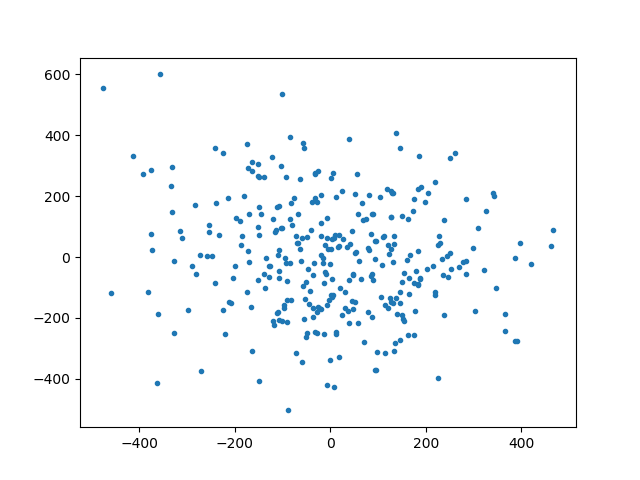
\includegraphics[scale=0.500000]{images/scopesim_templates_cluster.png}}\phantomsection\label{fig-scopesim-templates-cluster}

\caption{The positions of the cluster stars in arcseconds relative to the centre of the field of view .}
\end{figure}

\begin{enumerate}
\setcounter{enumi}{1}
\item A two component galaxy, with a younger component described by a star-forming spectra and an older by a
passive evolving spectral energy distribution
\end{enumerate}

\phantomsection\label{scopesim-templates-galaxy}
\begin{DUclass}{code}
\begin{DUclass}{plot}
\begin{DUclass}{clear-figure}
\begin{quote}
\begin{alltt}
\begin{lstlisting}[frame=single]
from scopesim_templates.basic.galaxy import spiral_two_component
import astropy.units as u

gal = spiral_two_component(fluxes=(20*u.ABmag, 21*u.ABmag))

plt.subplot(121)
plt.imshow(gal.fields[0].data)
plt.subplot(122)
plt.imshow(gal.fields[1].data)
\end{lstlisting}
\end{alltt}
\end{quote}
\end{DUclass}
\end{DUclass}
\end{DUclass}

\begin{figure}[H]
\noindent\makebox[\linewidth][c]{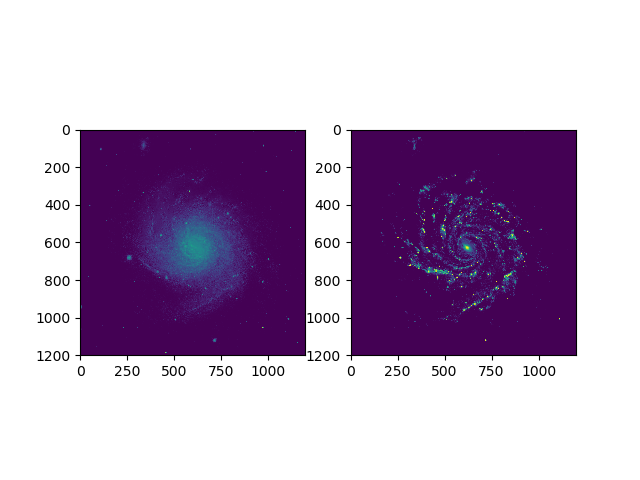
\includegraphics[scale=0.500000]{images/scopesim_templates_galaxy.png}}\phantomsection\label{fig-scopesim-templates-galaxy}

\caption{The two images which represent the new and old stellar populations of the spiral galaxy.}
\end{figure}

Above only the flux distribution on the sky can be appreciated. The description regarding the total flux
and its dependence with wavelength is contained in the \texttt{.spectra} property.

\phantomsection\label{scopesim-templates-galaxy-spectra}
\begin{DUclass}{code}
\begin{DUclass}{plot}
\begin{DUclass}{clear-figure}
\begin{quote}
\begin{alltt}
\begin{lstlisting}[frame=single]
gal = spiral_two_component(fluxes=(20*u.ABmag, 21*u.ABmag))
gal.spectra[0].plot(left=3000, right=8000, flux_unit="FLAM")
\end{lstlisting}
\end{alltt}
\end{quote}
\end{DUclass}
\end{DUclass}
\end{DUclass}

\begin{figure}[H]
\noindent\makebox[\linewidth][c]{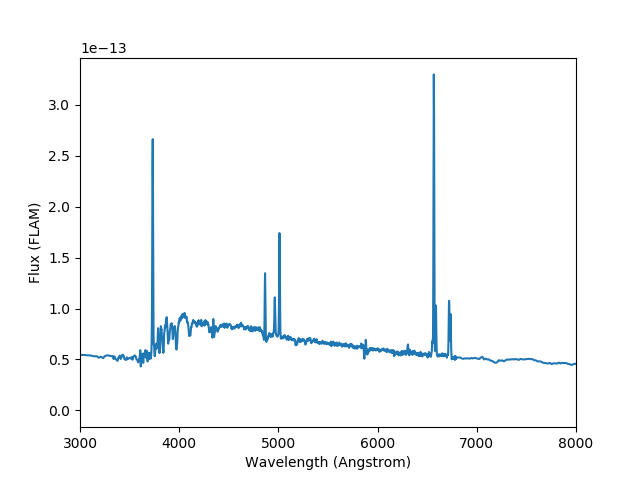
\includegraphics[scale=0.500000]{images/scopesim_templates_galaxy_spectra.png}}\phantomsection\label{fig-scopesim-templates-galaxy-spectra}

\caption{The spectra associated with each of the galaxy components}
\end{figure}


\subsection{Documentation%
  \label{documentation}%
}

\begin{itemize}
\item scopesim\_templates main documentation

\item source object interface documentation from scopesim-templates

\item converting from simcado to scopesim
\end{itemize}


%\chapter{The Instrument Reference Database}{IRDB: A collection of data for modelling each instrument with ScopeSim}

Documentation: \url{https://irdb.readthedocs.io/}

Code Base: \url{https://github.com/astronomyk/IRDB}

Continuous integration : \url{https://travis-ci.org/github/astronomyk/IRDB}

Author: Oliver Czoske


\section{What is contained in a packages%
  \label{what-is-contained-in-a-packages}%
}

Ascii, fits files
yaml config files

all effects
modes

how to define an effect via yaml


\section{Main packages vs support packages%
  \label{main-packages-vs-support-packages}%
}

\begin{itemize}
\item default.yaml

\item packages dependencies

\item modes\_yamls in default
\end{itemize}

all other yamls just have properties and effects


\section{List of available packages%
  \label{list-of-available-packages}%
}

% code for list_packages()


\section{Custom effects example%
  \label{custom-effects-example}%
}

\DUadmonition[warning]{
\DUtitle[warning]{Warning}

add code to show this (from astrometry notebook)
}


\section{Documentation%
  \label{documentation}%
}

\begin{itemize}
\item Reports of all packages

\item repo

\item tutorial on how to put together a package
\end{itemize}


%\chapter{AnisoCADO}


\section{AnisoCADO%
  \label{anisocado}%
}

A package for analytically generating SCAO PSFs primarily for the ELT

Documentation: \url{https://anisocado.readthedocs.io/}

Code Base: \url{https://github.com/astronomyk/AnisoCADO}

Continuous integration : \url{https://travis-ci.org/github/astronomyk/AnisoCADO}

Author: Kieran Leschinski


\subsection{Introduction%
  \label{introduction}%
}

\begin{itemize}
\item 
\begin{description}
\item[{Why AnisoCADO exists}] \leavevmode 
\begin{itemize}
\item Quickly create SCAO PSFs
\end{itemize}

\end{description}

\item 
\begin{description}
\item[{Limiting assumptions}] \leavevmode 
\begin{itemize}
\item Long exposure PSFs (> D\_M1 / v\_wind)

\item No coherence between time steps
\end{itemize}

\end{description}
\end{itemize}


\subsection{Examples%
  \label{examples}%
}

\begin{itemize}
\item Basic use case

\item Off-axis
\end{itemize}

\phantomsection\label{code-anisocado-example}
\begin{DUclass}{code}
\begin{DUclass}{execute}
\begin{quote}
\begin{alltt}
from anisocado import AnalyticalScaoPsf

psf = AnalyticalScaoPsf(N=64, wavelength=2.15)  # um
on_axis = psf.psf_on_axis
off_axis = psf.shift_off_axis(15, -5)   # arcsec
\end{alltt}
\end{quote}
\end{DUclass}
\end{DUclass}

% action: plot
% name: anisocado_basic_example
% ---
% plt.figure(figsize=(10,5))
% plt.subplot(121)
% plt.imshow(on_axis, norm=LogNorm())
% plt.subplot(122)
% plt.imshow(off_axis, norm=LogNorm())

\begin{figure}
\noindent\makebox[\linewidth][c]{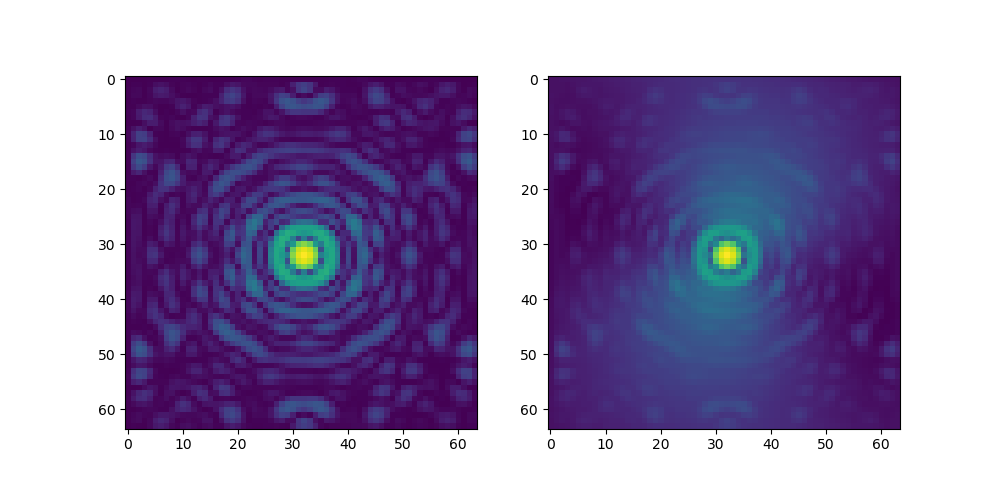
\includegraphics[scale=0.500000]{images/anisocado_basic_example.png}}\phantomsection\label{fig-anisocado-basic-example}

\caption{Left: the on-axis K-band (2.15\$mu\$m) SCAO PSF for standrard atmospheric conditions.
Right: the K-band SCAO-PSF at the position (15, -5) arcseconds from the natural guide star.}
\end{figure}


\subsection{Functionality%
  \label{functionality}%
}

\begin{itemize}
\item How AnisoCADO creates the SCAO PSFs

\item Long / Short exposure PSFs

\item Off axis

\item Wavelength dependence
\end{itemize}


%\chapter{SkyCalc iPy}


\section{SkyCalc\_iPy%
  \label{skycalc-ipy}%
}

An interactive python wrapper for the ESO SkyCalc\_cli package

Documentation: \url{https://skycalc_ipy.readthedocs.io/}

Code Base: \url{https://github.com/astronomyk/skycalc_ipy}

Continuous integration : \url{https://travis-ci.org/github/astronomyk/skycalc_ipy}

Author: Kieran Leschinski


\subsection{Functionality%
  \label{functionality}%
}


\subsection{Examples%
  \label{examples}%
}


%\chapter{SpeXtra}

<One line summary here>

Documentation:

Code Base:

Continuous integration:

Author: Miguel Verdugo


\section{Functionality%
  \label{functionality}%
}


\section{Examples%
  \label{examples}%
}


%\chapter{Pyckles}

A python package for quick easy access to the Pickles (1998) catalogue

Documentation: \url{https://skycalc_ipy.readthedocs.io/}

Code Base: \url{https://github.com/astronomyk/skycalc_ipy}

Continuous integration : \url{https://travis-ci.org/github/astronomyk/skycalc_ipy}

Author: Kieran Leschinski


\section{Functionality%
  \label{functionality}%
}

\begin{itemize}
\item accessing as if spectra are properties

\item multiple spectral libraries available
\end{itemize}


\section{Examples%
  \label{examples}%
}

\begin{itemize}
\item Pickles spectra in various formats

\item Brown spectra
\end{itemize}



\end{document}
